
\section{Motivation}

Knowing your machine is a major advantage when trying to optimize high-performance scientific code. \iaca\ \cite{iaca} is a tool by Intel to analyze \emph{X86} machine code with respect to a specific microarchitecture. However, it has some drawbacks that often times prevent it from being useful in practice. The main reason is that doesn't support the newest processors. \iaca\ $3.0$, which released in late 2017, supports the \nth{4} (Haswell) to the \nth{6} (Skylake) generation of Intel microarchitectures. Skylake was released in 2015. \iaca\ $2.3$ additionally supports the \nth{2} (Sandy Bridge) and the \nth{3} (Ivy Bridge) generation. So at the time of writing \iaca\ is about three years behind and further development remains unclear.\\
The second complication is that \iaca\ is closed source. Its user guide \cite{userguide} is the only documentation it has which provides little to no information about how it actually computes its output. As a result a user will often find himself wondering how its output fits the analyzed program.\\
In this work we present \suaca\ (Saarland University Architecture Code Analyzer), an open source alternative. It uses measurements provided by \cite{Andreas} which are parsed during runtime. This way a user doesn't rely on a software update of the tool as he can simply perform the measurements on his own, should we not already support his microarchitecture. Note that this is only possible with Intel architectures so far. At the time of writing \suaca\ supports all Intel microarchitectures from the \nth{1} (Nehalem) to the \nth{8} (Coffee Lake) generation, except for the server variant of Skylake.

\newpage
\section{Scope of work}

Like mentioned before we will present a tool that is able to analyze given \emph{X86} assembler code in respect to a specific microarchitecture. Just like \iaca\ our tool is able to find byte markers inside a compiled file and analyze the code in between. Those markers can be inserted in two different ways: inserting them by hand in the assembler code or use the \emph{iacaMarks.h} header in your \emph{C} code. First take a look at the assembly variant:

\begin{mdframed}[backgroundcolor=light-gray, roundcorner=10pt,leftmargin=1, rightmargin=1, innerleftmargin=15, innertopmargin=1,innerbottommargin=1, outerlinewidth=1, linecolor=light-gray]
\begin{lstlisting}[language={myLang}]
 movl $111, %ebx
.byte 0x64, 0x67, 0x90

    //Some code here
    
 movl $222, %ebx
.byte 0x64, 0x67, 0x90
\end{lstlisting}
\end{mdframed}

\iaca\ is mainly used to analyze critical parts of scientific code, which are usually inside a loop. When using a loop in \emph{C} code one can easily insert the markers defined in the \emph{iacaMarks.h} header like this:

\begin{mdframed}[backgroundcolor=light-gray, roundcorner=10pt,leftmargin=1, rightmargin=1, innerleftmargin=15, innertopmargin=1,innerbottommargin=1, outerlinewidth=1, linecolor=light-gray]
\begin{lstlisting}
#include "iacaMarks.h"

int main(void) {

    while (condition) {
        (*@\textcolor{Green}{IACA\_START}  @*)
        //Some code here
    }
    (*@\textcolor{Green}{IACA\_END}  @*)

    return 0;
}
\end{lstlisting}
\end{mdframed}

In both cases a user has to compile his code and run \suaca\ on the compiled file. We are using Intel's \emph{X86 Encoder Decoder
} library \cite{xed} to disassemble said file, which allows us to support files of the \emph{ELF}, \emph{PECOFF} and \emph{MACHO} format.\\
After disassembling \suaca\ will perform a dependency analysis on the instructions and parse the measurement file. Finally it will perform a simulation of the code. It won't consider the actual effect of the instructions, only their latencies, dependencies and port usage. The instructions are first considered in program order, although instruction reordering is still possible as we will see in \autoref{sec:chooseport}. For several reasons, which we will discuss in the following, our simulation will compute an estimate of the code's performance, not total numbers.\\
\suaca\ is able to perform several kinds of analyses which we will discuss in \autoref{chap:functionality}. In \autoref{chap:algorithms} we will then explain in detail how the most important parts of the simulation and the dependency analyzes are done.


\section{Intel's microarchitectures}


\begin{wrapfigure}[25]{l}{0.6\textwidth}
    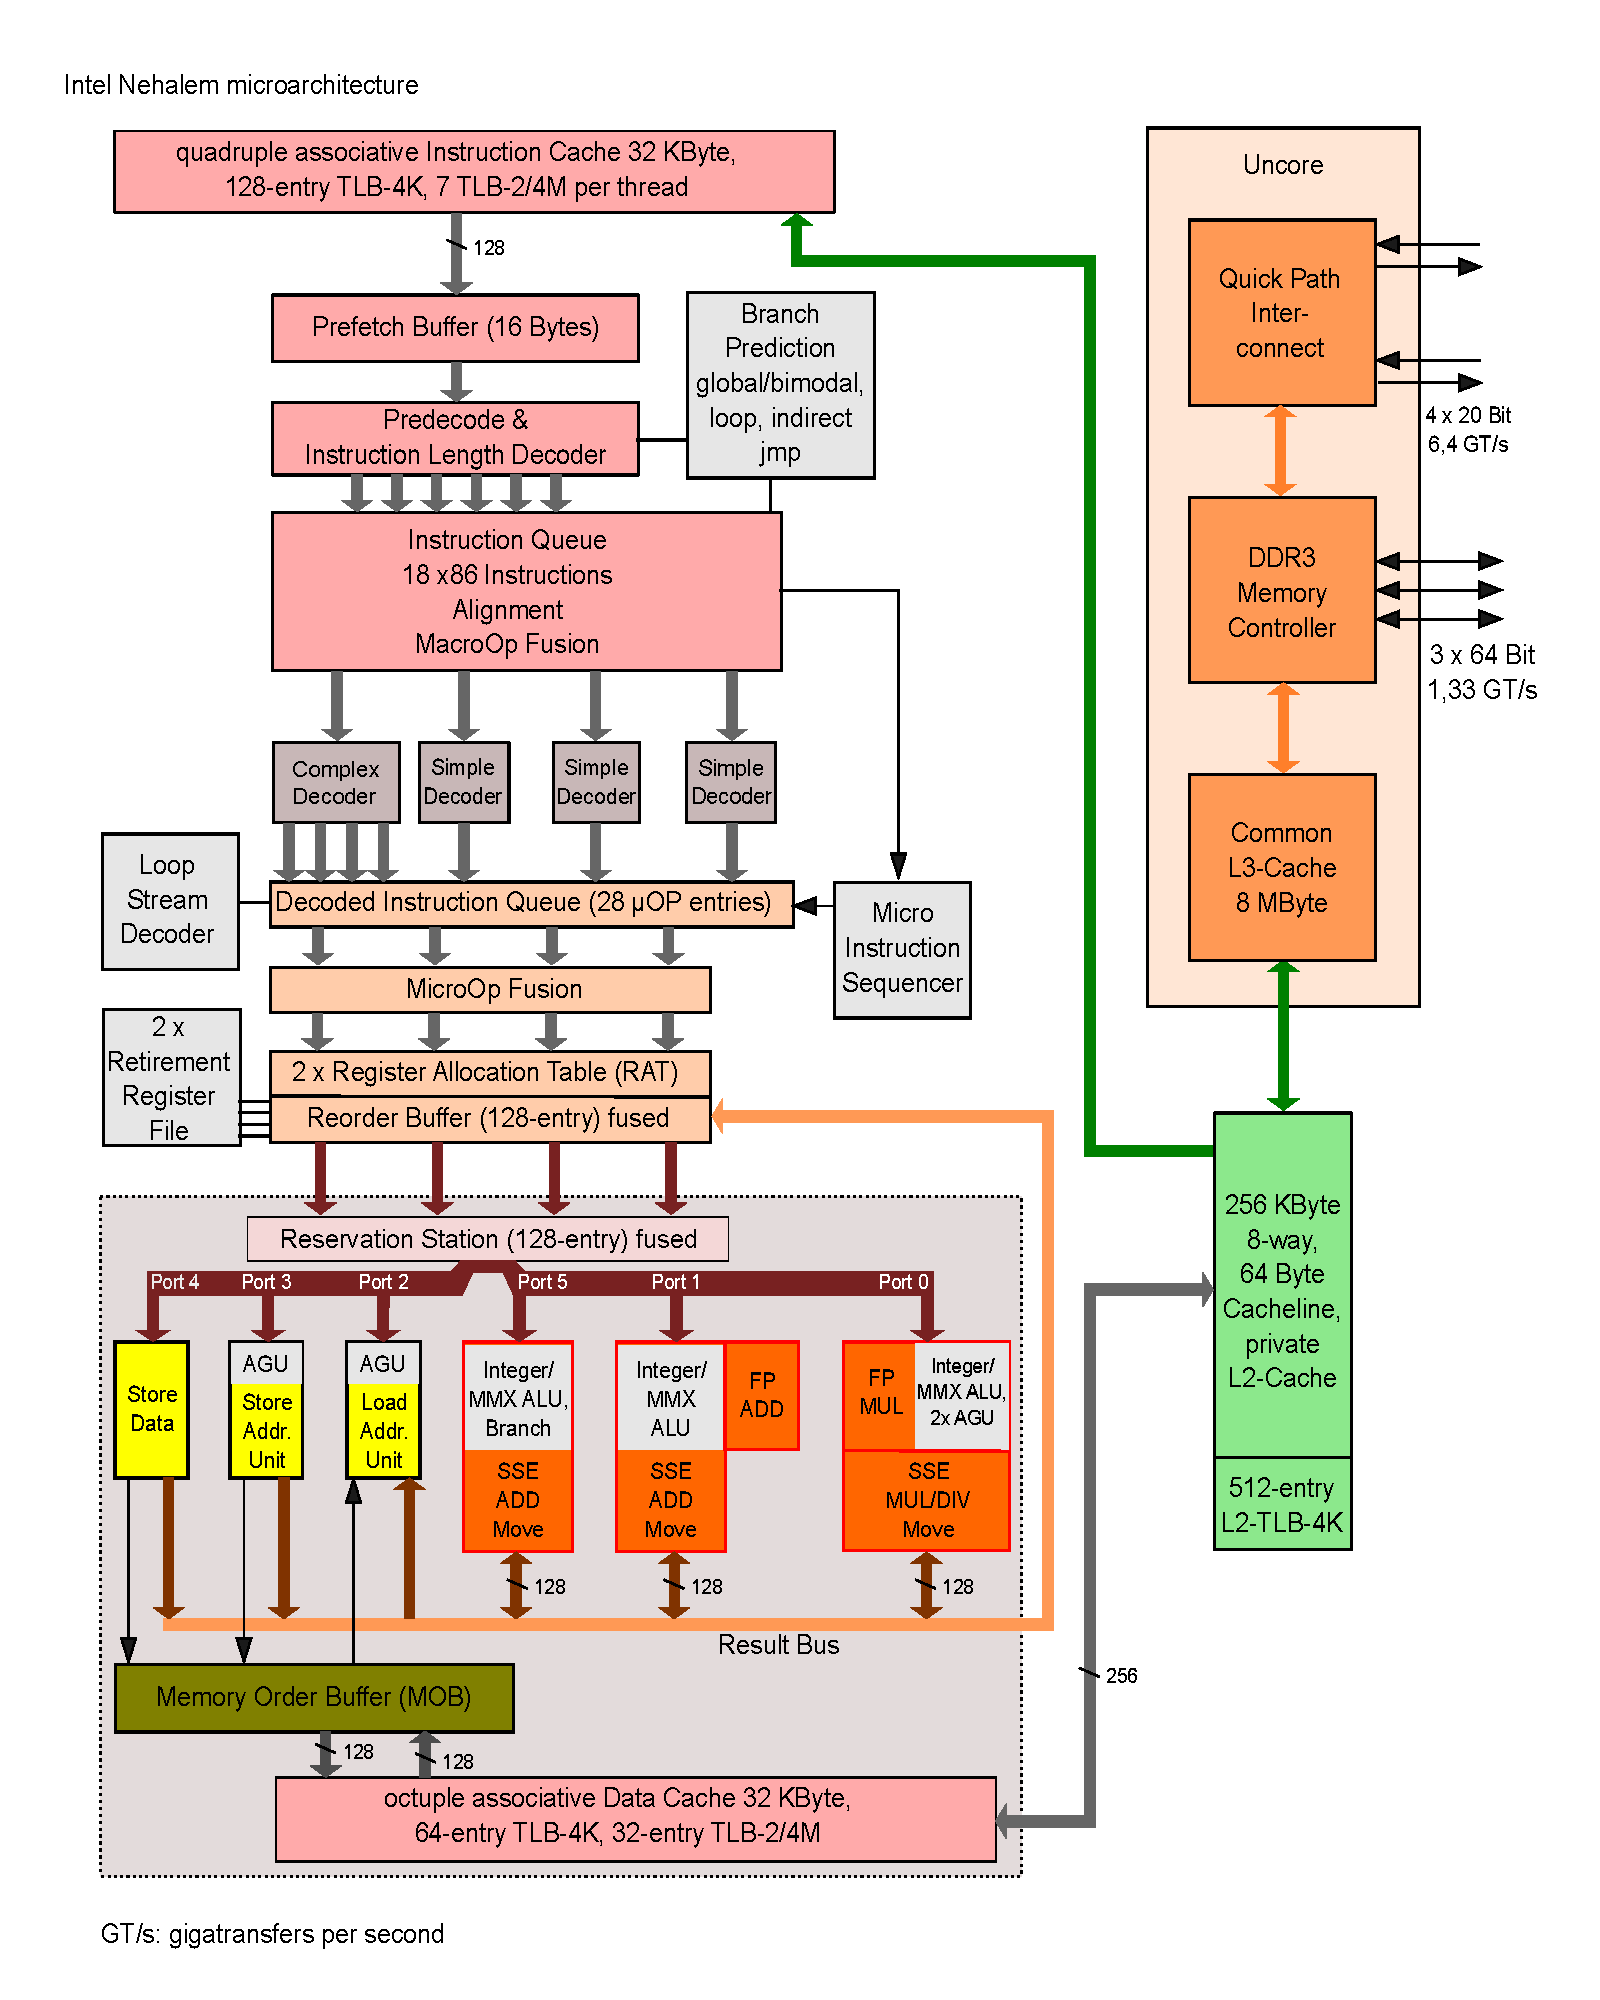
\includegraphics[width=0.6\textwidth]{Intel_Nehalem_arch}
    \caption{Intel Nehalem architecture \cite{nehalem}}
    \label{fig:NHMfull}
\end{wrapfigure}


In order to understand some of our computations one also needs some basic knowledge about Intel's microarchitectures. They use the \emph{X86} instruction set. However, they don't execute those instructions directly. They will translate them into a sequence of so called \microops, which can then be executed. Unfortunately there is little to no documentation about those \microops, neither about the functionality of an individual one nor about their interaction with each other. From our measurements we can conclude that each microarchitecture has its own \microops which makes it even harder to find reliable information.\\ \autoref{fig:NHMfull} shows a sketch of the Nehalem architecture. We can see the decoders which are responsible for the translation of the \microops, but most of this sketch is not of particular interest for us. In our simulation we will consider most of this as the ``front end'' which will only be simulated by the number of \microops\ it produces each cycle. Our main interest lies in the gray dotted rectangle shown by \autoref{fig:NHMdetail}.\\
This figure shows the reservation station (or scheduler). It is responsible for the distribution of the \microops\ over the ports. As mentioned before, each cycle a certain amount of those will be loaded into the reservation station.


\begin{wrapfigure}[15]{r}{0.6\textwidth}
    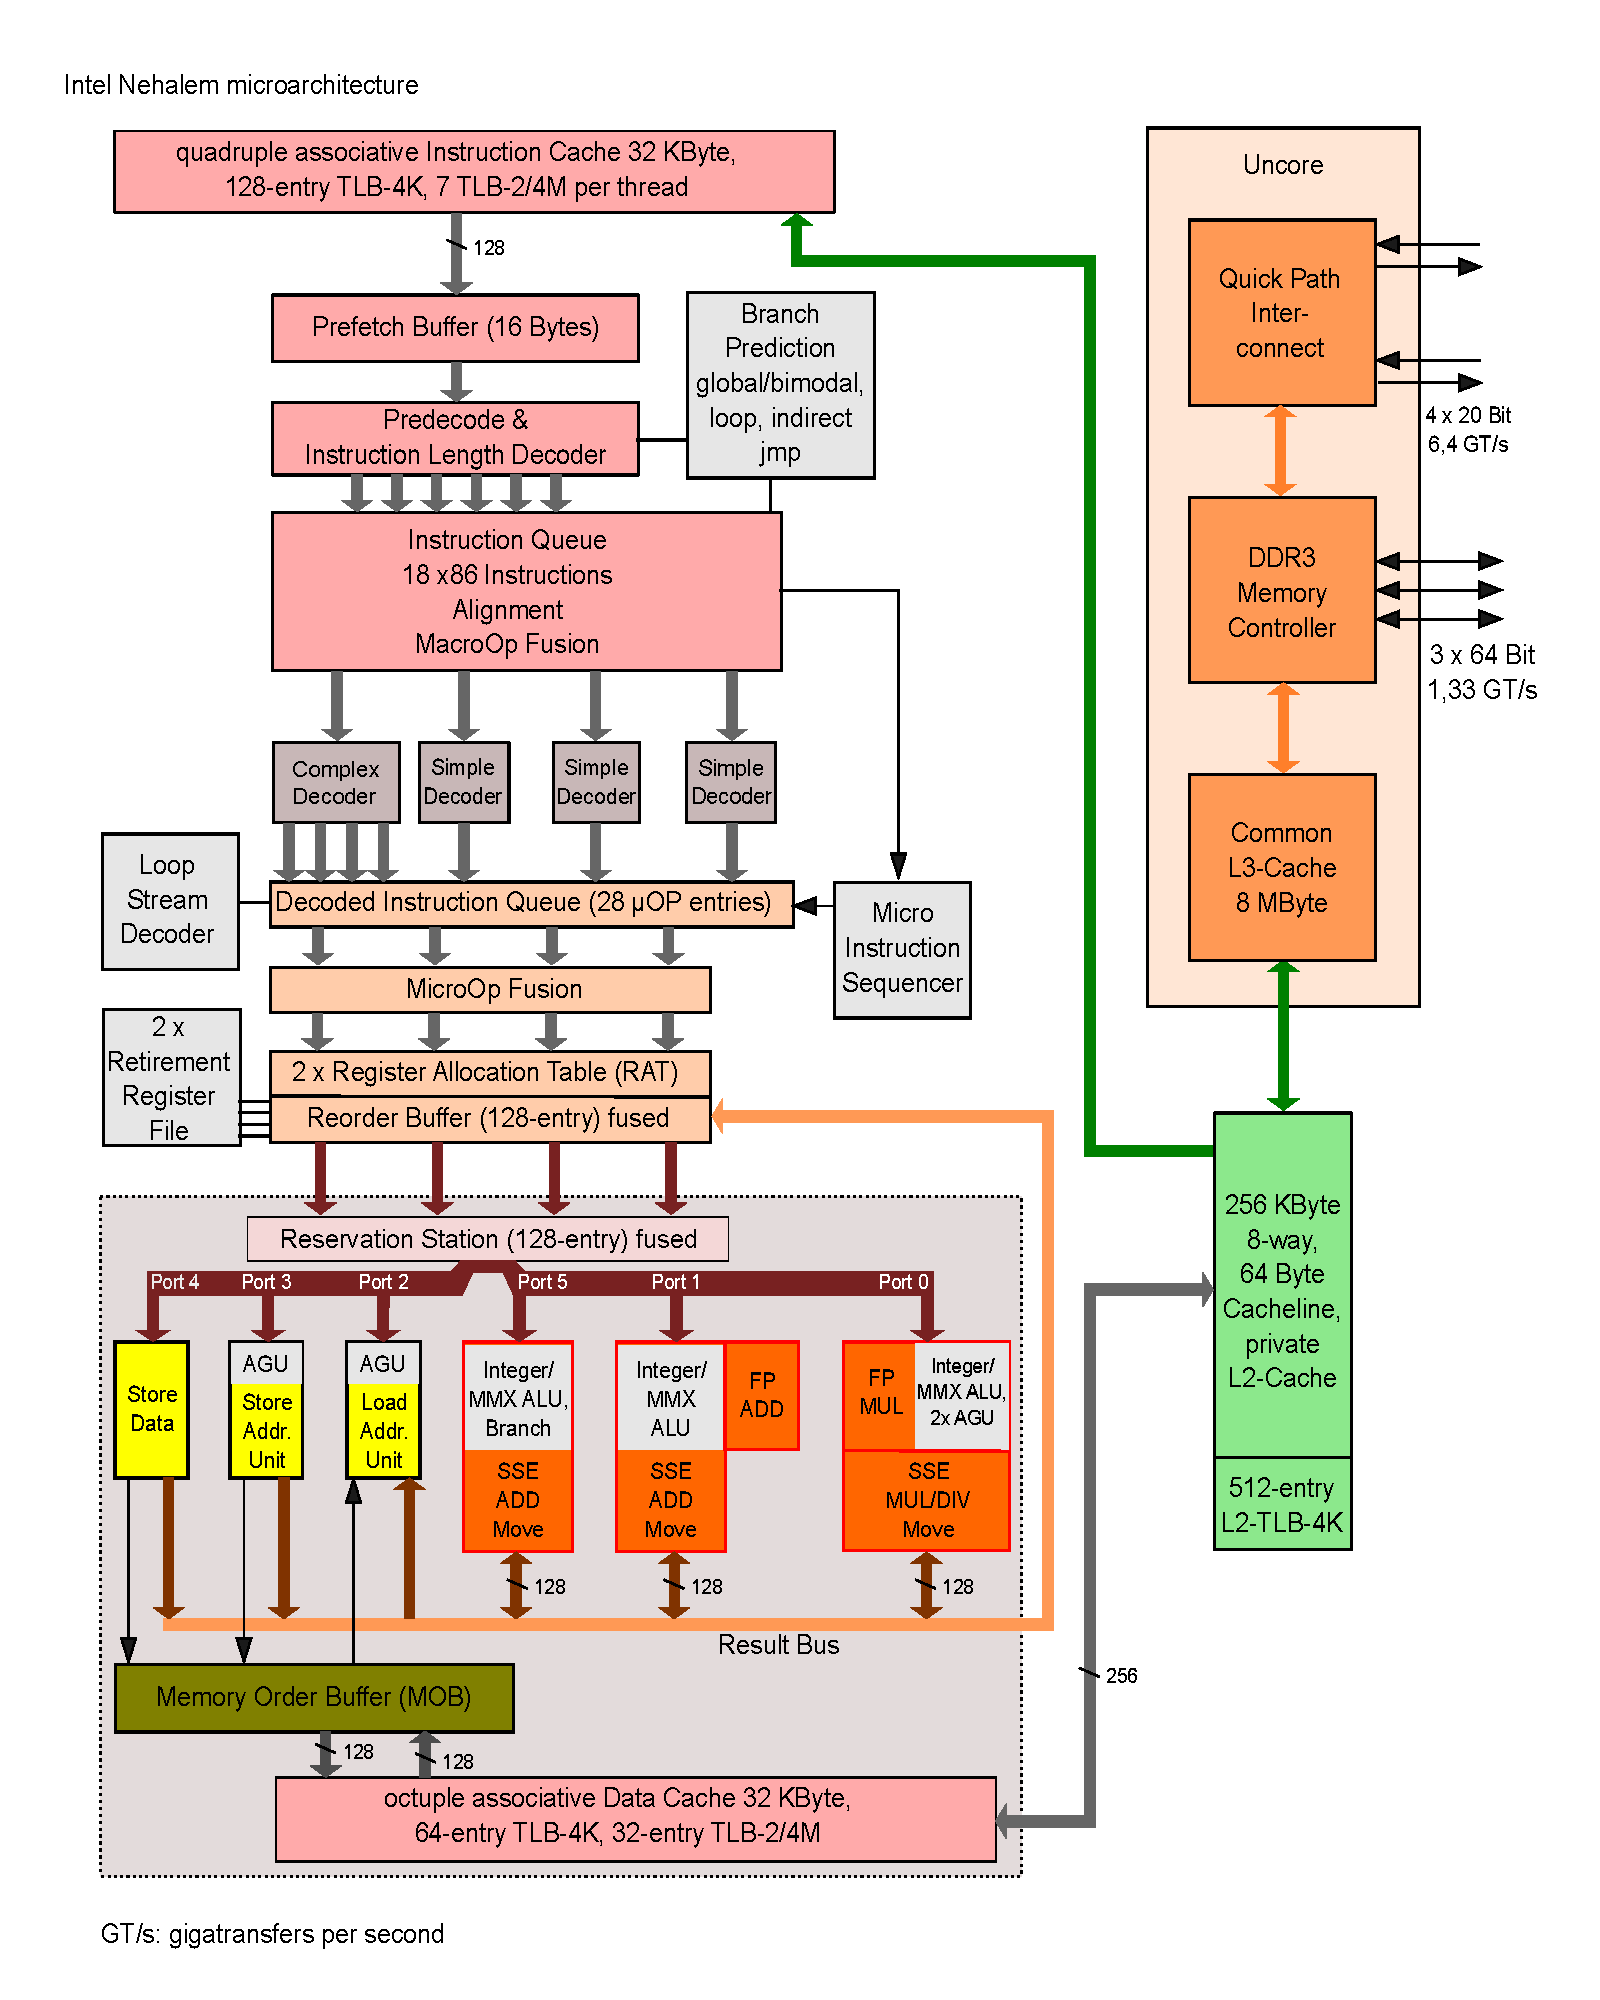
\includegraphics[clip, trim=0.5cm 2cm 9.78cm 20cm,width=0.6\textwidth]{Intel_Nehalem_arch}
    \caption{Detailed view \cite{nehalem}}
    \label{fig:NHMdetail}
\end{wrapfigure}

 How many depends on the architecture, in the case of Nehalem it's $4$. The capacity also depends on the specific architecture. The important property we can observe from this figure are the ports. Each port can be seen as a pipeline that a \microop\ can run through in order to be executed. On the ports themselves lie the actual execution units of the processor like the \emph{ALU}, \emph{MULTIPLEXER} and so on. Every port can hold a single \microop\ per cycle and they support pipelining. So they will be free again in the next cycle. The only exception from this is the \emph{DIVIDER} unit which is slow at executing and can block a port for multiple cycles.

\section{Measurements}
\label{sec:measurements}

As mentioned before a crucial part of \suaca's functionality are the measurements provided by \cite{Andreas}. Consider this snippet from the XML-measurement-file file:


\begin{lstlisting}[language=XML, basicstyle=\ttfamily\scriptsize, breaklines=false]
<instruction ... iform="ADD_LOCK_MEMv_GPRv" ...>
    <operand idx="2" type="reg" ...>RAX,RCX,RDX,RBX,...</operand>
    <operand idx="3" type="flag" ...>OF</operand>
    <operand idx="4" type="flag" ...>SF</operand>
    ...
    <architecture name="NHM">
        <measurement port15="2" port2="1" port3="1" port4="1" total_uops="5">
            <latency cycles="19" ... targetOp="3"/>
            <latency cycles="19" ... targetOp="4">
            ...
        <\measurement>
    </architecture>
<\instruction>
\end{lstlisting}

We dotted out some unnecessary or redundant information. As we can see in the first line this is the information for the instruction with the \emph{iform} ``ADD\_LOCK\_MEMv\_GPR''. \emph{iform} is an enum from the XED Library (\cite{xed}) that is used to identify instructions. We can extract the following information from our snippet:

\begin{itemize}
    \item One of the \emph{RAX, RCX, RDX, \dots} registers is an operand and they have the id $2$. We only need the mapping of $id \rightarrow register$ here as the xed library will tell us which operands are actually used in the analyzed programs. Similarly the flags also have their ids. The flags are the single bits of the \emph{RFLAGS} register in \emph{X86}.
    \item We have some measurements for the intel nahelem architecture.
    \item When simulating NHM the instruction consists of $5$ \microops. Two of which can use ports $1$ and $5$. One each can use port $2$, port $3$ and port $4$.
    \item It will take $19$ cycles to compute the result for the operand with id $3$. Most instructions have several latency items, depending on the number and kind of operands. In our case there is no information for operand $2$ as the instruction won't write to those registers. However, the latency for the operand with id $4$ is also $19$ cycles. Some instructions actually produce their results in a specific order. It might be that one operand is available after $3$ cycles and another one after $5$, so an instruction that only needs the first of those operands has to wait $3$ cycles whereas another one that needs the second operand has to wait $5$. \suaca\ can simulate this behavior as it knows which operand is causing the dependency. When simulating the whole instruction \suaca\ takes the maximum of those values. Note that those values are always best case, i.e.\ no port was blocked and no dependency occurred.
\end{itemize}


\section{Related work}

Like mentioned before one can find general information about \iaca\ at its website \cite{iaca}. The user's guide \cite{userguide} gives additional information about the usage and provides some examples. \iaca\ is developed by Israel Hirsh and Gideon S.\\

Andreas Abel \cite{Andreas} provides the measurements which enable us to compute our results.\\

Jan Laukemann \cite{osaca-thesis} implemented an open source alternative to \iaca\ called \osaca\ \cite{osaca-web}. It relies on the measurements provided by Johannes Hofmann \cite{ibench}. We will discuss the difference between the three tools in \autoref{chap:eval}.
